\documentclass{report}


\usepackage{graphicx}

% Puts the abstract on the title page
\usepackage{titling}
\newsavebox{\abstractbox}
\renewenvironment{abstract}
 {%
  \global\setbox\abstractbox=\vtop\bgroup
  \begin{center}\bfseries\abstractname\end{center}%
 }
 {\par\egroup}
\renewcommand{\maketitlehookd}{%
  \par\vfil
  \box\abstractbox
}

% Changes the formatting of the chapter numbers
\usepackage{titlesec}
\titleformat{\chapter}
  {\normalfont\LARGE\bfseries}{\thechapter}{1em}{}
\titlespacing*{\chapter}{0pt}{3.5ex plus 1ex minus .2ex}{2.3ex plus .2ex}


% TITLE DATA
\title{Development of a Visible-NIR Photoluminescence Microspectrometer}
\author{Zach Colbert}
\date{Spring 2019}


\begin{document}
  % TITLE PAGE
  \begin{titlingpage}
    \begin{abstract}
      This is the abstract. It comes later.
    \end{abstract}
    \maketitle
  \end{titlingpage}


  \tableofcontents


  \chapter{Introduction}
  % \section{The Need for a Simpler Spectrometer (Motivation)}

Photoluminescence (PL) is the process by which materials will absorb a photon, exciting an electron to a higher-energy "excited state," then emit a photon as the electron relaxes back to a lower-energy state. Measuring PL in different ways is a common method for characterizing semiconducting materials.

Basic PL measurements are emission and excitation, and differ by their independent variables. Emission measurements use one wavelength to excite the material, and measure the intensity of light emitted across a chosen spectrum. Excitation measurements use many wavelengths to excite the material, and measure the intensity of light emitted at a particular wavelength. This project is centered around PL emission measurements.

The Micro-Femto Energetics ($\mu fE$) group at Oregon State University uses advanced optoelectronic methods to characterize materials, especially thin-layer materials and micron-scale semiconducting devices.

The group's workhorse when it comes to PL measurements is a Horiba \textbf{Something?} fluorimeter, coupled to a \todo{model?} microscope. The instrument uses a \todo{specs?} xenon-arc lamp and double-monochromator to illuminate a wide field with a tunable wavelength. The light source is coupled to the microscope with a fiber optic cable. The instrument can be configured for reflection or transmission microscopy depending on the application. With the aid of computer software, the instrument is able to measure both PL emission and excitation. However, there are a few distinct challenges to using this instrument.

Because the fiber optic delivers a large beam, a large area on samples is illuminated whether the instrument is in a reflection or transmission mode. The wide-field illumination is excellent for imaging, but makes it hard to isolate emissions from small spatial domains.

\todo{Something about the system takes a long time to warmup before the light source is stable.}

\todo{Check specs for monochromator. What is it's spectrum like vs. laser diode? More or less monochromatic?}

\todo{Something about training time and the learning curve for using the device. Software is kinda complicated. Takes a really long time to take a measurement.}

This project offers a solution to these challenges by designing and assembling a new PL microspectrometer that can measure the PL emission of samples accurately, quickly, and with the ability to illuminate small spatial domains.

Naturally, the new instrument has fewer applications. It only measures emission (not excitation), and reconfiguration for other measurements requires more consideration to optical design. The goal of this project, however, is to design an instrument that is simple to use for PL measurement when use of the fluorimeter is impractical, too time consuming, or the instrument is in use for another experiment.


  \chapter{Background}
  \subsection{Optoelectronic Materials}\label{chap:intro-optomats}

Optoelectronic materials convert light to electric energy and/or electric energy to light. The study of these materials goes back as far as the early 1900s, but accelerated rapidly in the 1960s with the advent of the light emitting diode and semiconductor laser \cite{sweeney_optoelectronic_2017}. Optoelectronic devices are ubiquitous; they have enabled the rapid growth of information technologies around the world, and are fundamental in modern telecommunication and internet infrastructure. Modern optronics research explores new materials that can be used to create faster, more efficient, and smaller optoelectronic devices.

\subsubsection{Organic Photovoltaic: ADT}\label{chap:intro-optomats-adt}

Organic optoelectronic materials are not a new discovery; however, they have become increasingly popular in recent decades as methods for creating them have advanced \cite{ostroverkhova_organic_2016}. The Ostroverkhova group at Oregon State University has studied several organic photovoltaics (OPVs) including functionalized derivatives of pentacene, benzothiophene, and anthradithiophene (ADT) \cite{e._b._shepherd_effect_2011, platt_optical_2009}. A drop-cast sample of fluorinated ADT with triethylsilyethynyl (TES) functional group, provided by the Ostroverkhova group, is used for demonstration of the new microspectrometer device in Chapter \ref{chap:results}.

\begin{figure}[H]
    \centering
    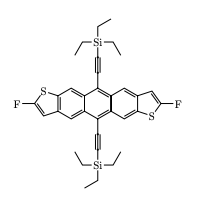
\includegraphics{img/adt-tes-f.png}
    \caption[Molecular diagram of ADT TES-F.]{Molecular diagram of fluorinated anthradithiophene (ADT) with triethylsilyethynyl (TES) side group. A drop-cast sample of this molecule was provided by the Ostroverkhova group at Oregon State University, and used for demonstration of our microspectrometer instrument following a study by Lam \cite{lam_polarization_2018}.}
    \label{fig:adt-diagram}
\end{figure}

\subsubsection{Quantum Dots: \ce{CdSe}}\label{chap:intro-optomats-qd}

Quantum dots (QDs) are artificial semiconductor particles, typically only a few nanometers in size. There has been a fair amount of research on the tunability of optoelectronic properties in QDs by varying their size and shape. Quantum dots have many of the same potential applications as other optoelectronic materials but are attractive for their size and reproducibility. Previous studies have shown how quantum dots can be produced en masse with a high degree of control over their shape and size \cite{empedocles_photoluminescence_1996, murray_synthesis_2000}.

A sample of CdSe quantum dots, suspended in solution and drop-cast on a glass slide, is used to demonstrate the new microspectrometer device in Chapter \ref{chap:results}.

\subsection{Mechanics of Photoluminescence}
Photoluminescence occurs in molecules where the valence and conduction bands are separated by a small band gap near the Fermi level. A molecule absorbs a photon with energy greater than or equal to its band gap, exciting an electron from its ground state in the valence band to an excited state in the conduction band. The electron lives in this excited state for a short time, and then relaxes back to the ground state.

The electron can relax non-radiatively --- losing energy as it transitions through vibrational modes --- or radiatively, losing a small amount of energy to vibrational transitions and then returning to the ground state. When it returns to the ground state, the energy is emitted as a photon. We expect the energy of this photon to be lower than that of the absorbed photon (and the wavelength longer) because of the loss of energy to vibrational transitions.

% Because of the loss of energy to vibrational transitions, we expect the energy of this photon to be lower than that of the absorbed photon, and the wavelength longer.

Measurement of fluorescent emissions yields information about the energy of these electron transitions, allowing us to map out the electron band structure of molecules.


  \chapter{Design}
  % \input(chapters/design.tex)

  \chapter{Results}
  In general, results from the microspectrometer are much smoother than results from the fluorimeter, which include quite a lot of noise. We suspect that this is a consequence of wide-field illumination used by the fluorimeter, in which molecules outside the region of interest (or otherwise, with some defects) are excited and emit spectra different from that of the region of interest. \todo{Instead of this, explore power dependence. Need sources. Have some questionably reliable data for the laser, no data for the Horiba. Can I get some generic data for Horiba to compare?}

\subsection{ADT TES-F}

\begin{figure}[h]
    \centering
    \begin{subfigure}[b]{0.45\textwidth}
        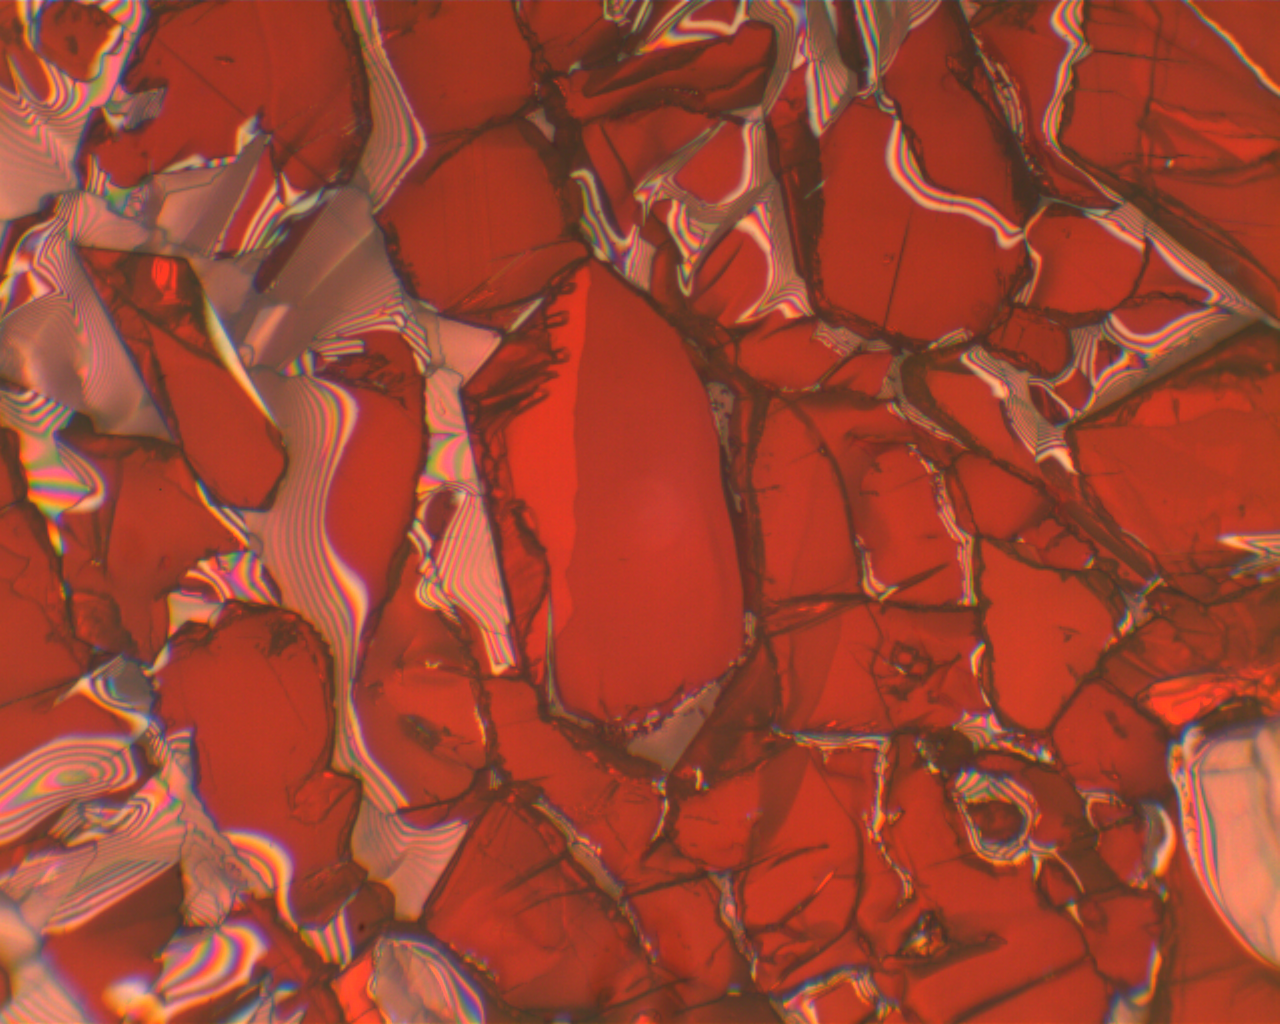
\includegraphics[width=\textwidth]{./img/tesf-white-illum.png}
        % \caption{TESF region of interest under white light.}
        \caption{}
        \label{img:tesf-white}
    \end{subfigure}
    \hfill
    \begin{subfigure}[b]{0.45\textwidth}
        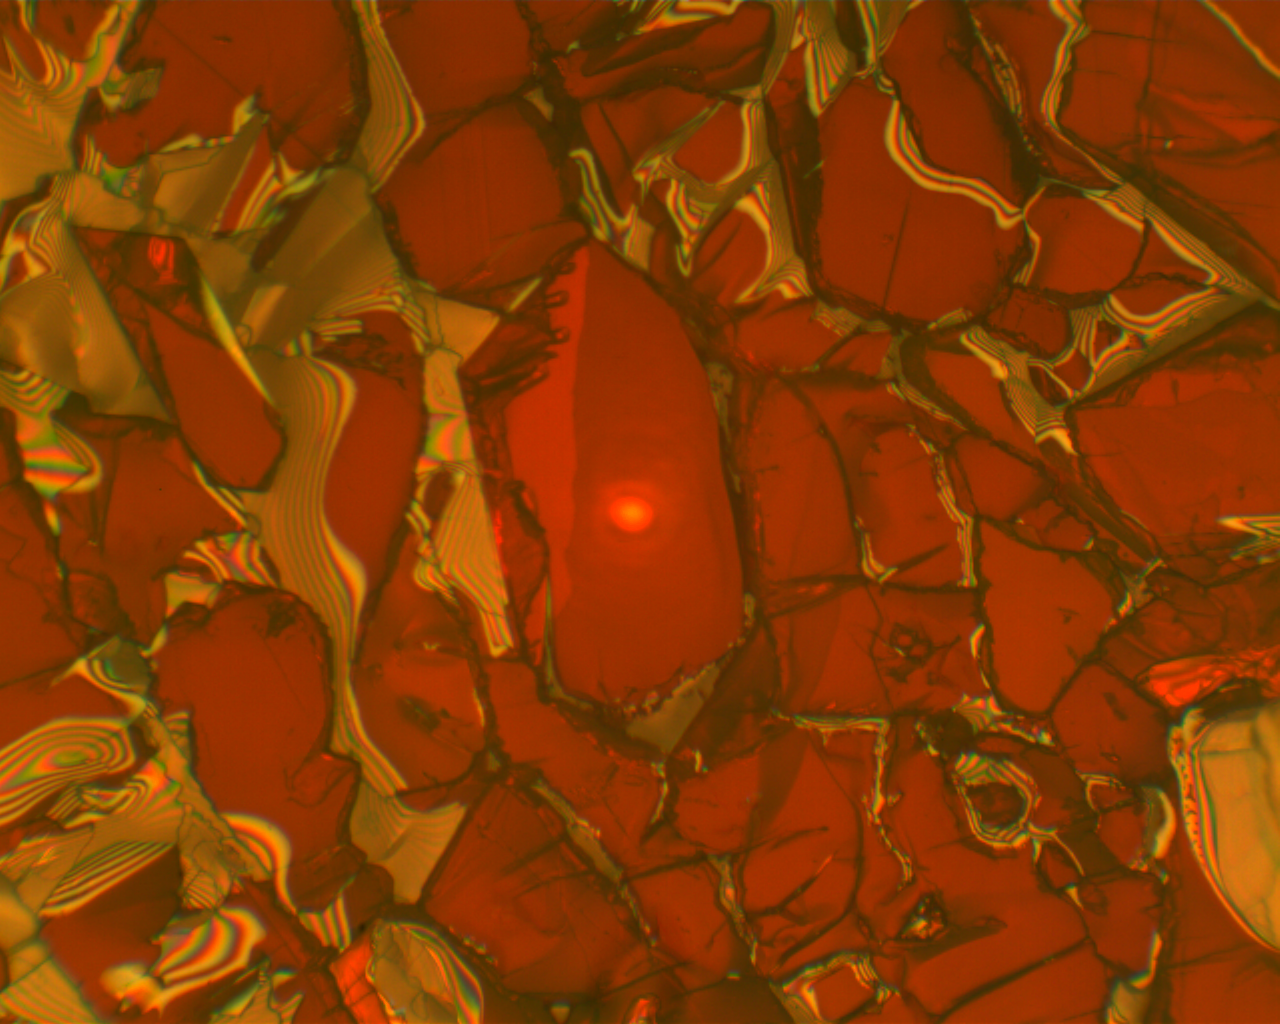
\includegraphics[width=\textwidth]{./img/tesf-laser-illum.png}
        % \caption{TESF region of interest under excitation light.}
        \caption{}
        \label{img:tesf-laser}
    \end{subfigure}
    \caption{Images of ADT TES-F sample under white light (\ref{img:tesf-white}) and under laser excitation light (\ref{img:tesf-laser}). Photoluminescence spectra of this region are shown in Figure \ref{fig:pl-adt-tesf}.}
    \label{img:tesf}
\end{figure}

For a drop-cast sample of ADT TES-F on glass, we selected a region of interest which appeared to be a single crystal, with few visually distinguishable defects (Figure \ref{img:tesf}). The crystal was also selected such that its surface area was larger than the area illuminated by the microspectrometer's laser spot. The emission spectra of the region of interest are shown in Figure \ref{fig:pl-adt-tesf}.

\todo{Convert wavelength from nm to eV? This seems to be a more common unit in solid state.}

Both spectra in Figure \ref{fig:pl-adt-tesf} show a clear peak around 630nm, which has been shown in other research.\cite{lam_polarization_2018}\cite{ostroverkhova_organic_2016}\cite{platt_optical_2009} The spectra measured by the microspectrometer also shows a secondary peak just below 600 nm, which is not evident in the spectrum taken by the fluorimeter. \note{All 3 citations in this paragraph have spectra with peaks similar to mine, but different intensity. This must be because they excited at a different wavelength, but how do I use that?}

\begin{figure}[h]
    \centering
    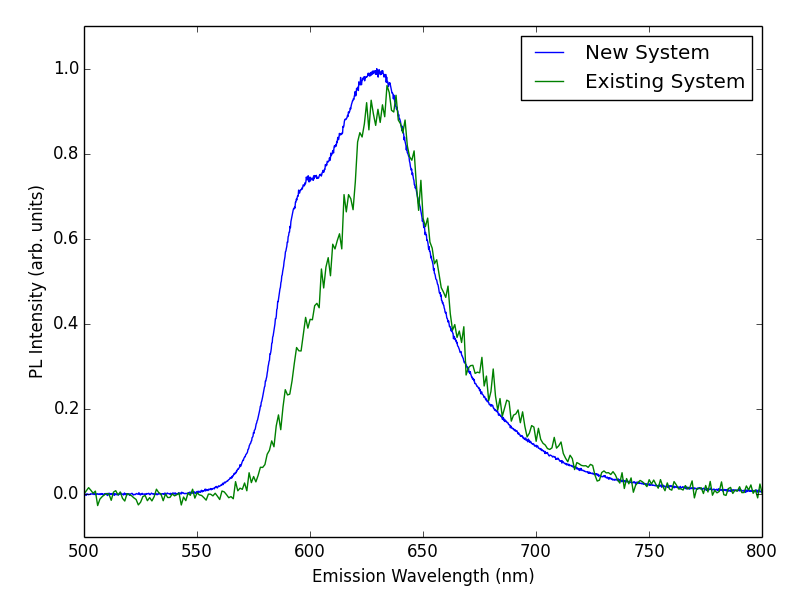
\includegraphics[width=.8\textwidth]{./img/tesf-2.png}%\llap{\raisebox{4cm}{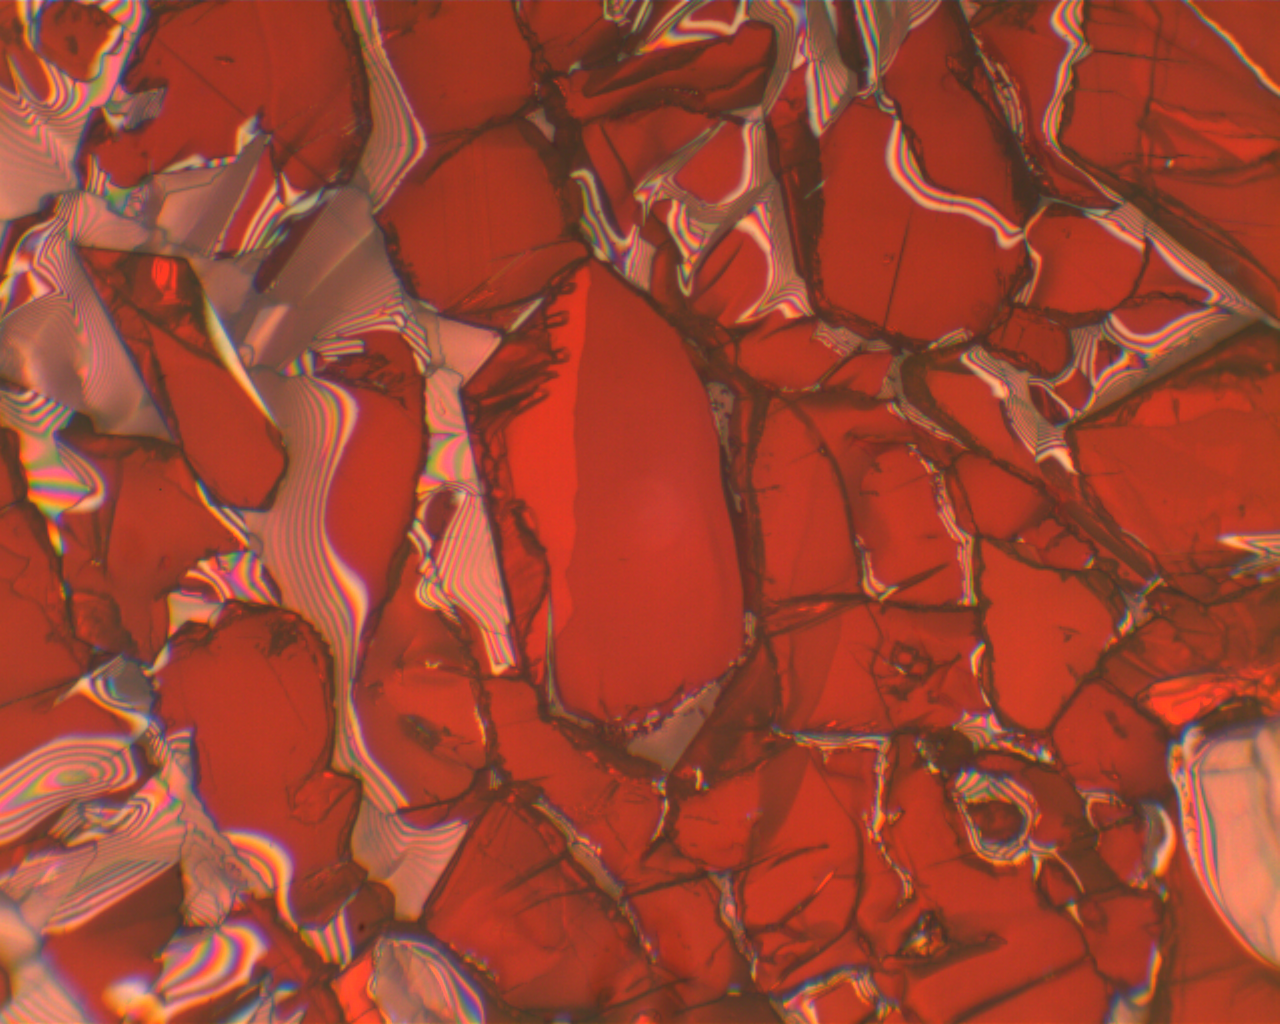
\includegraphics[width=2cm]{img/tesf-white-illum.png}}}
    % 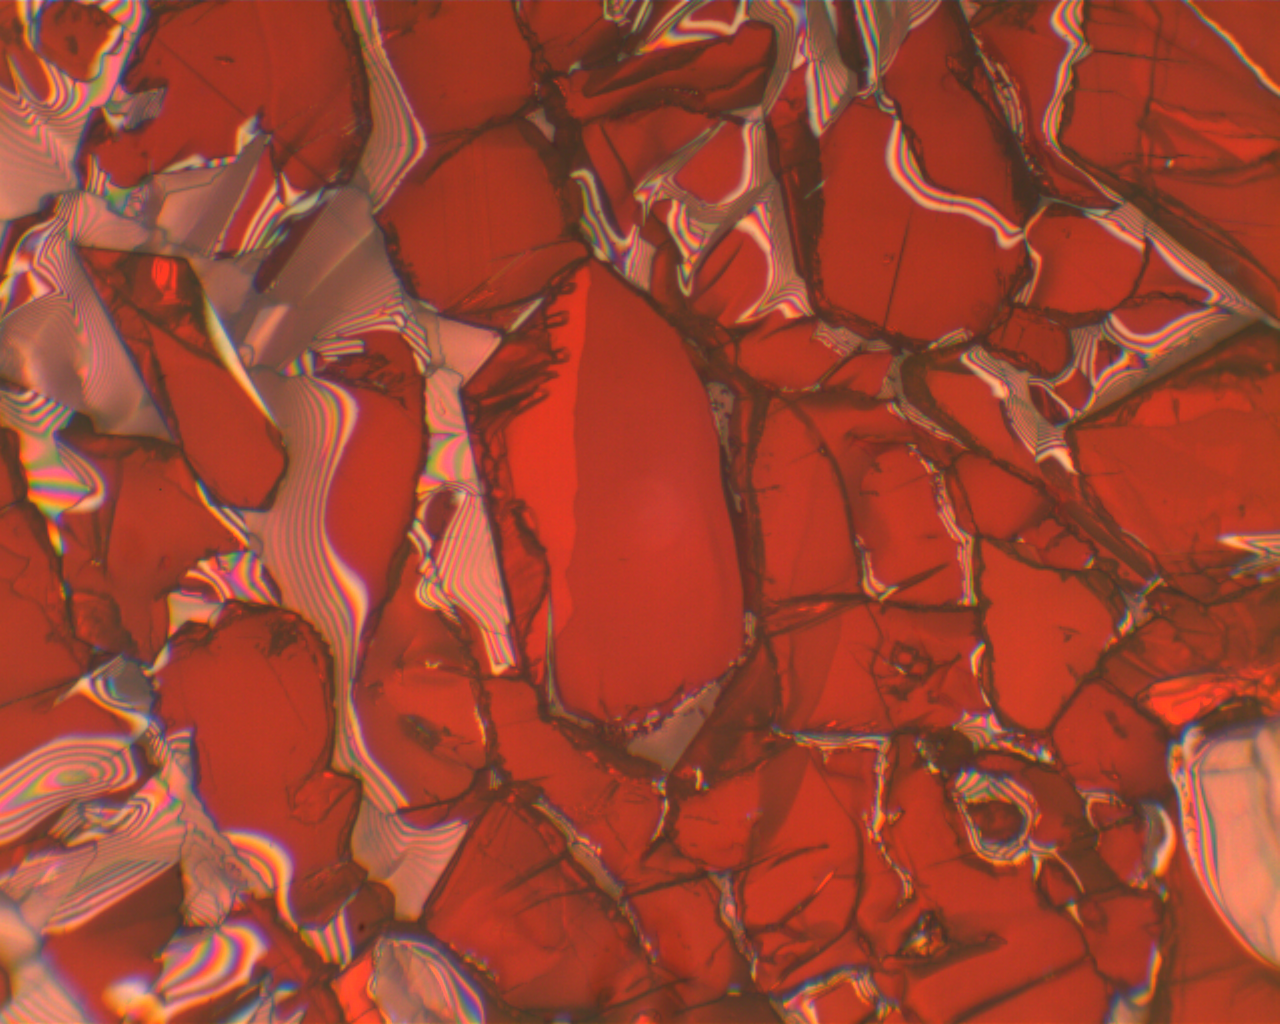
\includegraphics[width=.2\textwidth]{./img/tesf-white-illum.png}
    % 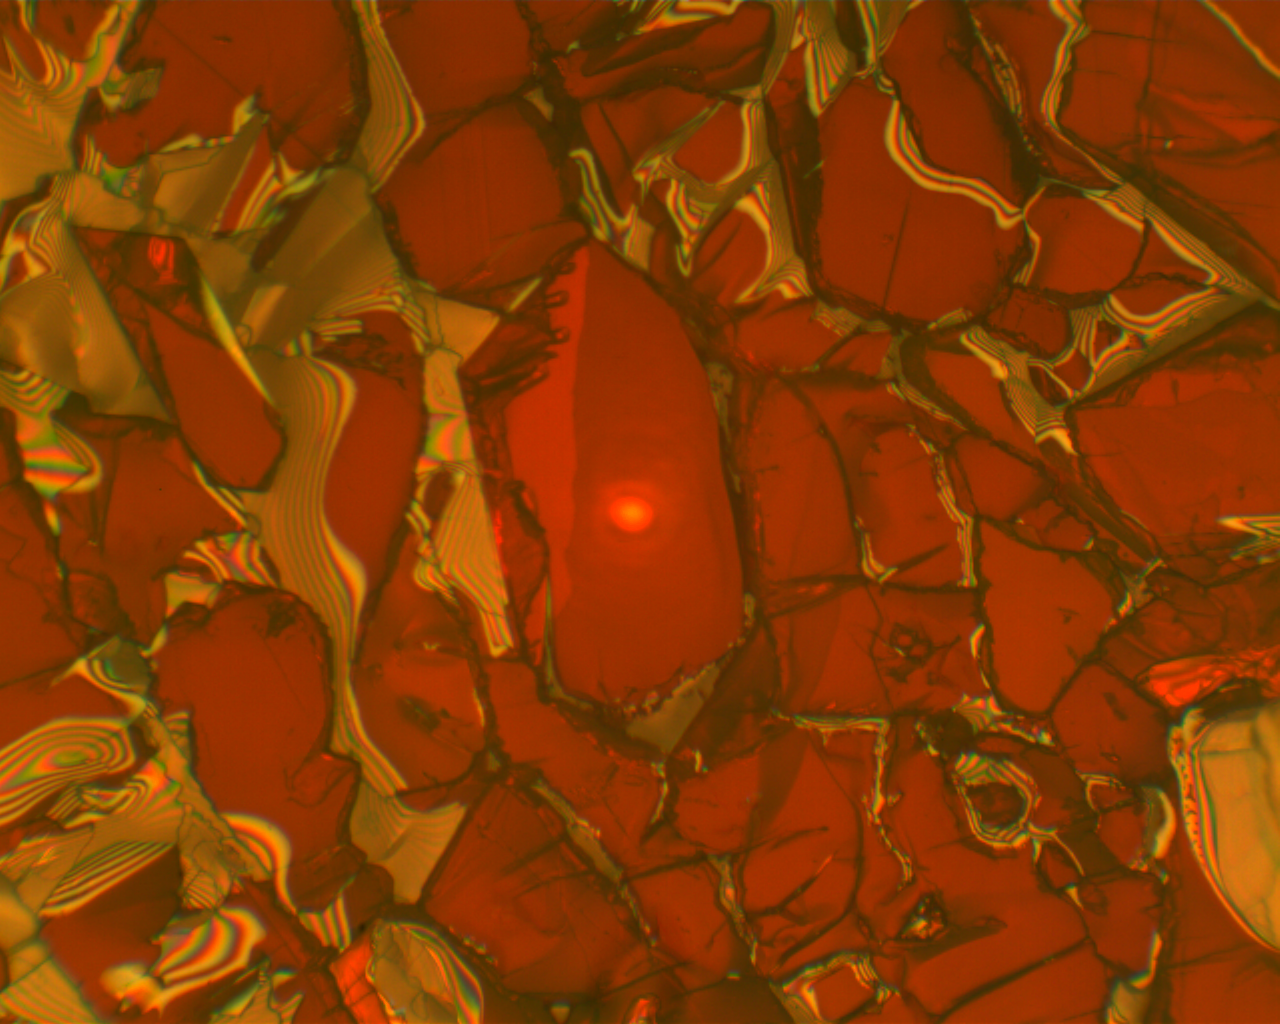
\includegraphics[width=.2\textwidth]{./img/tesf-laser-illum.png}
    \caption[PL emission spectrum of ADT TES-F, excited at 405nm.]{PL emission spectrum of ADT TES-F, excited at 405 nm.
    Wide-field illumination used by the existing system to excite the sample
    yields a noisy spectrum, and does not excite the secondary peak that is 
    shown clearly in the results from the new system. A single crystal, larger than the laser spot, was selected among smaller neighboring crystals for this measurement. %This may be because the
    %wide-field illumination is exciting many adjacent crystals in the sample, 
    %which emit slightly different spectra. The laser illumination in the new 
    %system has the spatial resolution necessary to illuminate single crystals.
    }
    \label{fig:pl-adt-tesf}
\end{figure}

\subsection{\ce{CdSe} Quantum Dots}

\begin{figure}[h]
    \centering
    \begin{subfigure}[b]{0.45\textwidth}
        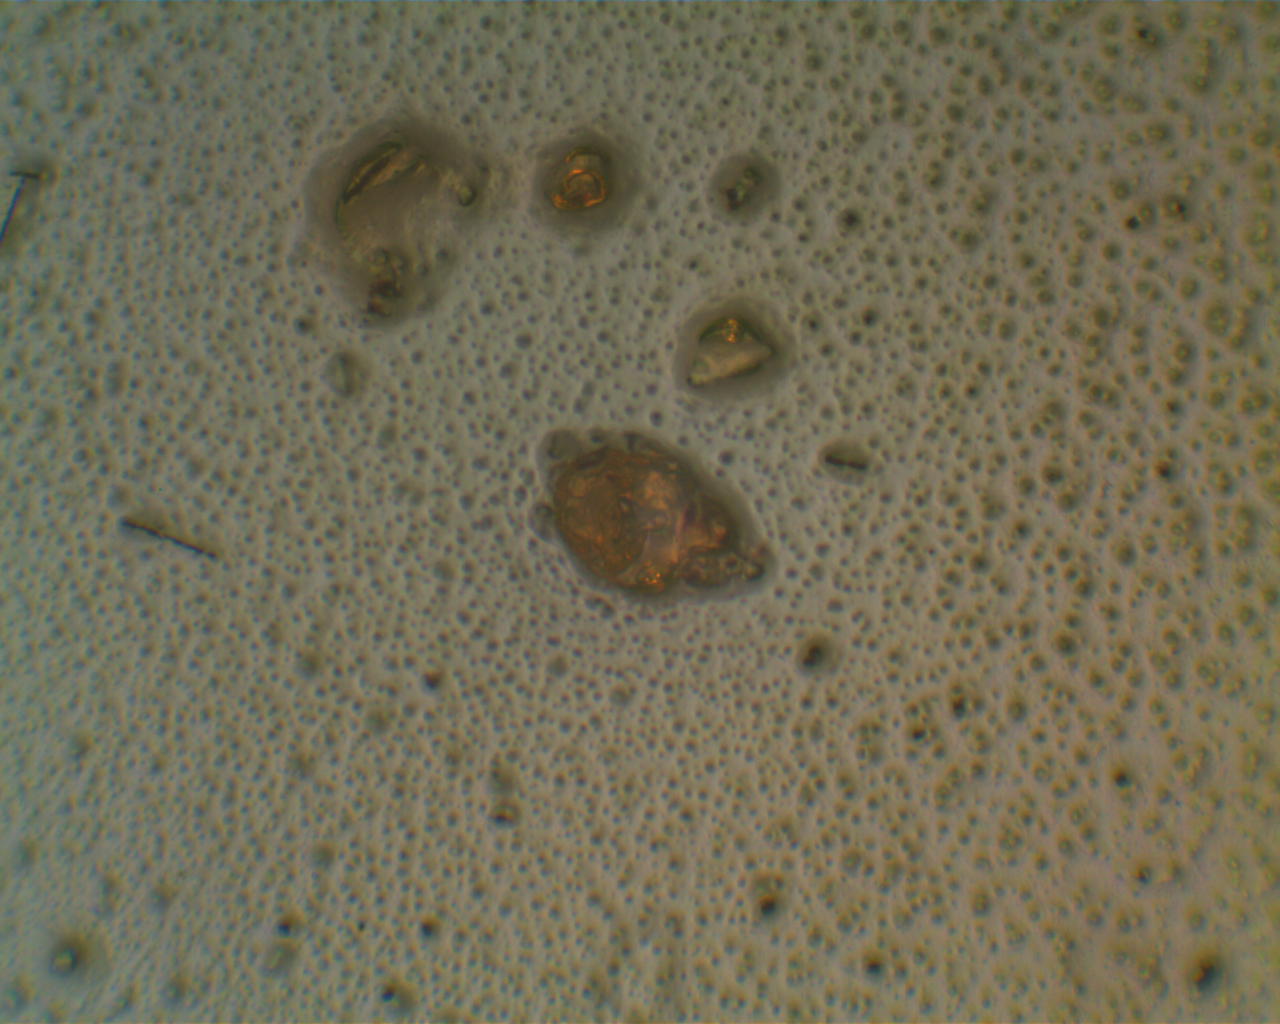
\includegraphics[width=\textwidth]{./img/qd-white-illum.png}
        \caption{}
        \label{img:qd-white}
    \end{subfigure}
    \hfill
    \begin{subfigure}[b]{0.45\textwidth}
        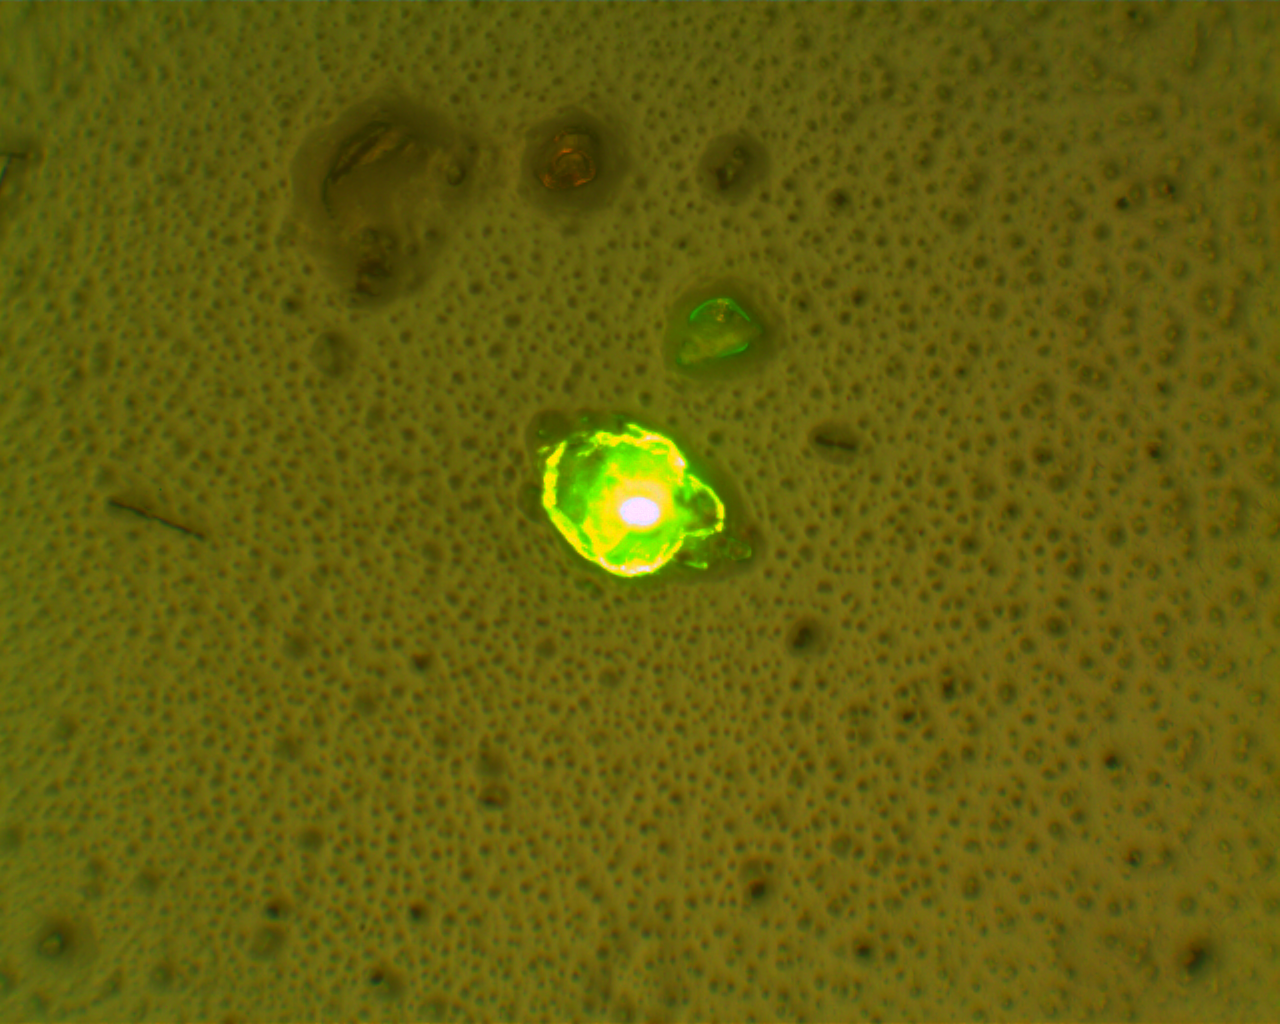
\includegraphics[width=\textwidth]{./img/qd-laser-illum.png}
        \caption{}
        \label{img:qd-laser}
    \end{subfigure}
    \caption{Images of CdSe quantum dot sample under white light (\ref{img:qd-white}) and under laser excitation light (\ref{img:qd-laser}). Photoluminescence spectra of this sample are shown in Figure \ref{fig:pl-adt-qd}.}
    \label{img:qd}
\end{figure}

Figure \ref{fig:pl-adt-qd} shows the PL emission of CdSe quantum dots \todo{on what substrate?}. There is one broad, clear peak that aligns well with the same measurement taken on the fluorimeter, between 520 and 620 nm. This peak seems to agree with other studies of CdSe quantum structures.\cite{empedocles_photoluminescence_1996}

Unlike the same measurement taken on ADT, this measurement was taken in a region of interest which is sparsely populated with quantum dots, with one target grouping illuminated by the laser.

\todo{What else do I write about here? Need to find more resources on analysis of PL, i.e. what information we get about the material. This will also be useful for Background section.}

\begin{figure}[h]
    \centering
    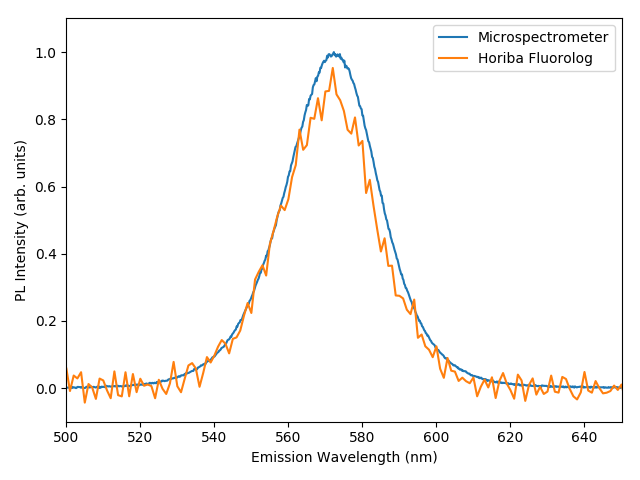
\includegraphics[width=\textwidth]{./img/qd-2.png}
    % 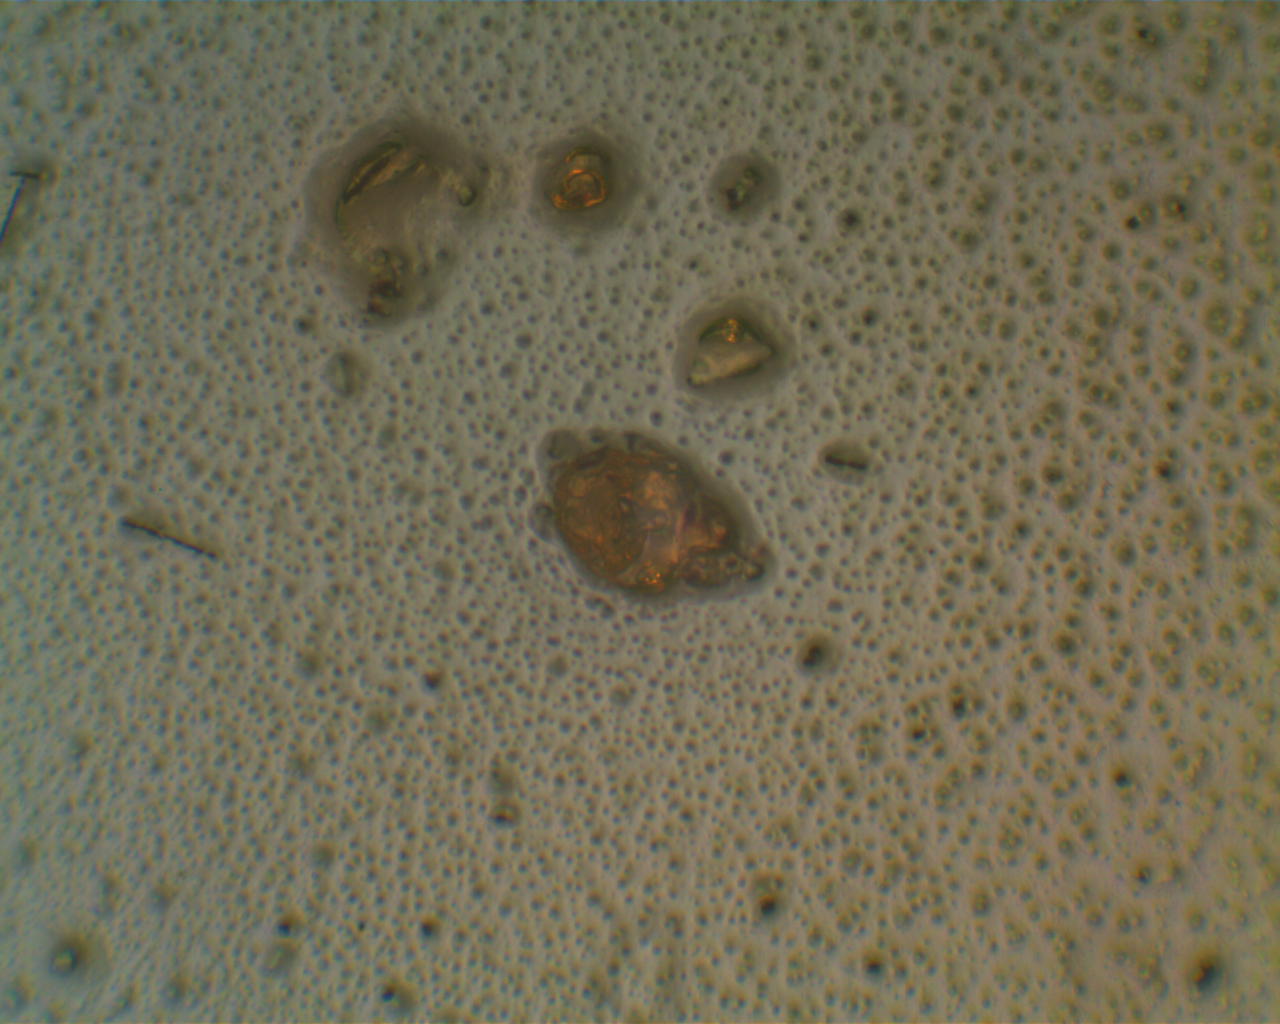
\includegraphics[width=4cm]{./img/qd-white-illum.png}
    % 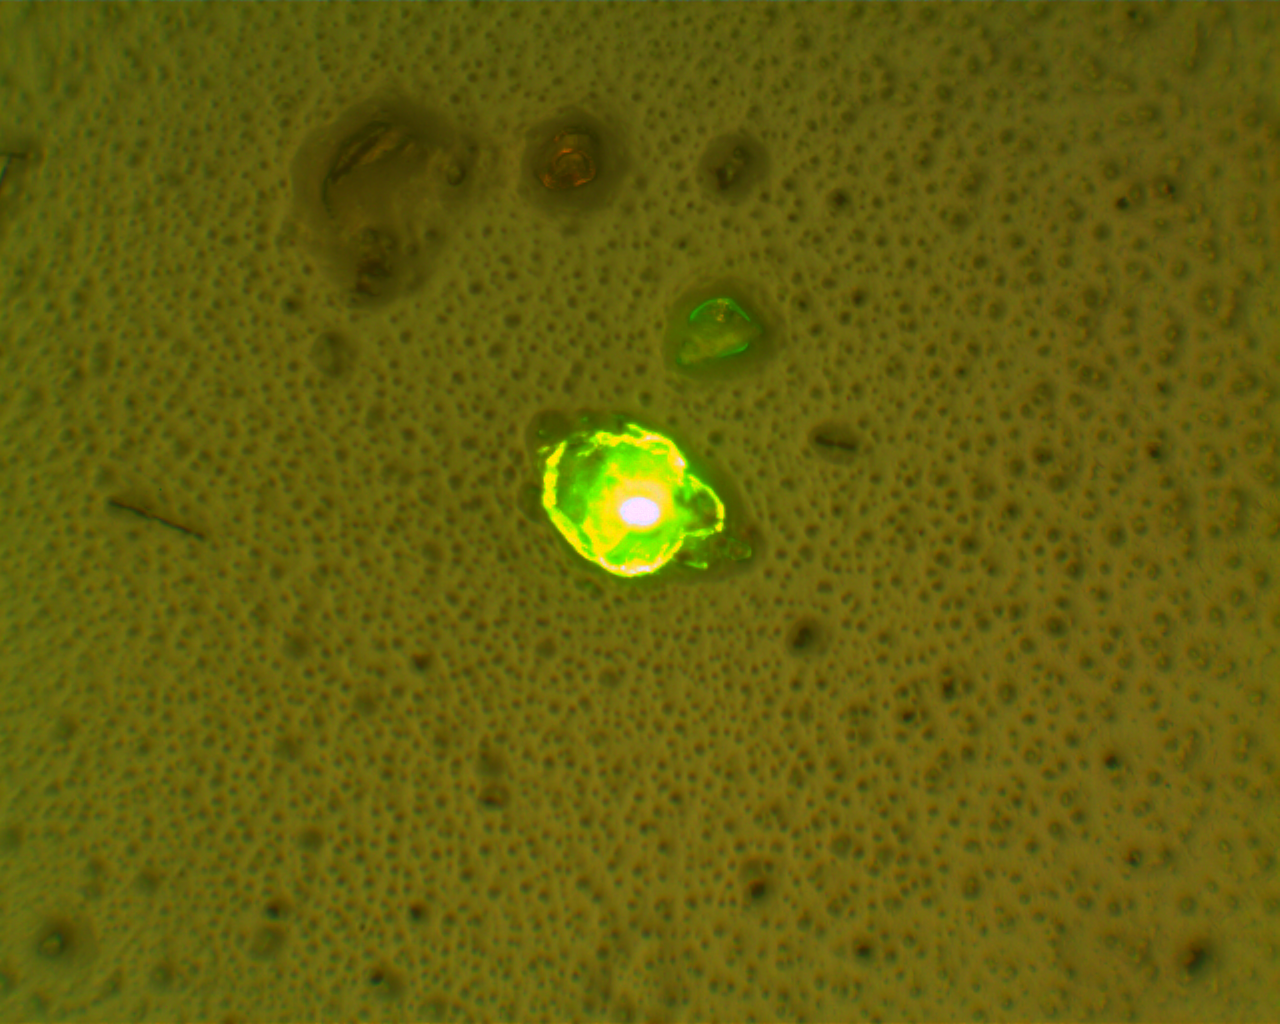
\includegraphics[width=4cm]{./img/qd-laser-illum.png}
    \caption{PL emission spectrum of a cluster of CdSe quantum dots on ?? substrate, excited at 405 nm.}
    \label{fig:pl-adt-qd}
\end{figure}


  \chapter{Analysis}
  % \input(chapters/analysis.tex)

  \chapter{Conclusion}
  % \input(chapters/conclusion.tex)

  \chapter*{Acknowledgements}
  % \input(chapters/acknowledgements.tex)

  \chapter*{References}
  % \input(chapters/references.tex)


  \appendix
  \chapter{Code}
  % \input(appendix/code)

\end{document}